\documentclass{article} % Tạo một bản báo cáo
\usepackage[utf8]{inputenc}
\usepackage[T5]{fontenc} % Để sử dụng Tiếng Việt
\usepackage[fontsize=14pt]{scrextend} % Set fontsize=13pt
\usepackage[paperheight=29.7cm,paperwidth=21cm,right=2cm,left=3cm,top=2cm,bottom=2.5cm,twoside]{geometry} %căn lề các kiểu
\usepackage{amsmath}
\usepackage{amssymb}
\usepackage{graphicx} % Thư viện chèn ảnh
\usepackage{float} % Set vị trí chèn ảnh
\usepackage{tikz} % Thư viện tạo khung bìa
\usetikzlibrary{calc} % Thư viện tikz


\usepackage{indentfirst} % Thư viện thụt đầu dòng
\renewcommand{\baselinestretch}{1.2} % Giãn dòng 1.2
\setlength{\parskip}{6pt} % Spacing after
\setlength{\parindent}{1cm} % Set khoảng cách thụt đầu dòng mỗi đoạn
\usepackage{titlesec} % Thư viện để set up các kiểu chữ
\setcounter{secnumdepth}{4} % 4 Heading
\titlespacing*{\section}{0pt}{0pt}{30pt} % Heading 1
\titleformat*{\section}{\fontsize{16pt}{0pt}\selectfont \bfseries \centering}

\titlespacing*{\subsection}{0pt}{6pt}{0pt} % Heading 2
\titleformat*{\subsection}{\fontsize{14pt}{0pt}\selectfont \bfseries}

\titlespacing*{\subsubsection}{0pt}{6pt}{0pt} % Heading 3
\titleformat*{\subsubsection}{\fontsize{13pt}{0pt}\selectfont \bfseries \itshape}

\titlespacing*{\paragraph}{0pt}{0pt}{0pt} % Heading 4
\titleformat*{\paragraph}{\fontsize{13pt}{0pt}\selectfont \itshape}
\begin{document}
\section*{Lý thuyết}

\subsection*{Câu 2:}
Có 3 giả thuyết(assumption):
\begin{itemize}
    \item \textbf{Tính chuỗi markov (Markovianity):} 
    Trạng thái hiện tại của biến chỉ phụ thuộc vào trạng thái trước đó (của biến hidden)
    
    $\mathbb{P}[H_t = h_t | H_{1:t-1} = h_{1:t-1},O_{1:t} = o_{1:t}]$ =  $\mathbb{P}[H_t = h_t | H_{t-1} = h_{t-1}]$ \\$\forall h_t \in \mathbb{H}$
    
   - Hợp lý: 
   
   - Không hợp lý: Tâm trạng của ngày hiện tại (Buồn, vui,...) không chỉ phụ thuộc vào nhiều ngày trước đó chứ không chỉ một ngày
    
    \item \textbf{Tính độc lập đầu ra (Output independence):} Trạng thái hiện tại của biến quan sát chỉ phụ thuộc vào trạng thái hiện tại của biến hidden
    
     $\mathbb{P}[O_t = o_t | H_{1:t} = h_{1:t},O_{1:t-1} = o_{1:t-1}]$ =  $\mathbb{P}[O_t = o_t | H_{t} = h_{t}]$ $\forall o_t \in \mathbb{O}$
     
     - Hợp lý: Trên bàn ăn có một chiếc thìa và một đôi đũa. Khi chọn chiếc thìa sẽ có khả năng ăn súp cao hơn và khi chọn đũa sẽ có khả năng ăn thịt cao hơn.
     
     - Không hợp lý: 
    
    \item \textbf{Tính ổn định (Stationarity)} Các xác suất chuyển đổi độc lập với thời gian
    
     $\mathbb{P}[H_t = j | H_{t-1} = i]$ =  $\mathbb{P}[H_{t+s} = j | H_{t+s-1} = i]$ $\forall i,j \in \mathbb{H}$
     
     - Hợp lý: Ngày chủ nhật được nghỉ học => tâm trạng có khả năng vui hơn, ngày tiếp theo là thứ hai => tâm trạng có khả năng chán hơn. Điều này cũng lặp lại tương tự sau một tuần.
     
     - Không hợp lý: Ngày chủ nhật buồn vì mất chiếc xe đạp, hôm sau mẹ cho tiền mua chiếc xe mới => vui. Không hợp lý nếu nói rằng tuần sau mình cũng có tâm trạng tương
\end

\subsection*{Câu 4:}

\textbf{Mô tả:} 

\hspace{1cm}Thuật toán viterbi là một dạng thuật toán quy hoạch động để xác định xác suất ước tính tối đa của trạng thái ẩn (Hidden state) có khả năng xảy ra nhất từ Observations đã cho. Giảm thiểu số lượng tính toán bằng cách lưu trữ các giải pháp được lặp lại bằng các bảng hai chiều. Viterbi tạo ra một đường $X = (x_1,x_2,...,x_T)$ là một chuỗi các trạng thái ẩn (hidden states) với $x_n \in S = {s_1,s_2,...,s_K}$, S tạo ra các biến quan sát (observations) $Y = (y_1,y_2,...,y_3)$ với $y_n \in O = {o_1,o_2,...,o_N}$  (N là số biến quan sát được trong không gian quan sát O)

\hspace{1cm} Có hai ma trận được cho trước: 
\begin{itemize}
    \item Ma trận chuyển tiếp (Transition) có kích thước KxK, Transition[i,j] lưu trữ xác suất đi từ $S_i$ tới $S_j$
    
    \item "Emission matrix" (Emission) có kích thước KxN, Emission[i,j] lưu trữ xác suất mà $O_j$ xảy ra từ $ S_i$
\end{itemize}
 
 Giả sử có một mô hình Markov ẩn(HMM) với $\pi_i$ là ma trận khả năng khởi tạo (ma trận biểu thị khả năng của các State lúc khởi tọ), các ma trận S, Transition đã nêu như trên. $V_{t,k}$ là ma trận lưu xác suất của chuỗi có khả năng xảy ra cao nhất của biến quan sát (Observation) t ban đầu  và có k là trạng thái ẩn (State/hidden state) cuối cùng.
 
 Công thức quy hoạch động:
 
 \hspace{1cm} $V_{1,k} = P(y_1 | k).\pi_k,$
 
 \hspace{1cm} $V_{t,k} = max_{x \in S}(P(y_t | k).Transition_{x,k}.V_{t-1,x})$

Đường đi Viterbi  lưu lại với x được sử dụng trong công thức thứ 2 bên trên.Hàm Ptr(k,t) trả về giá trị x được chọn khi tính $V_{t,k}$

\hspace{1cm} $x_T = argmax_{x \in S}(V_T,x)$

\hspace{1cm} $x_{t-1} = Ptr(x_t,t)$

\textbf{Đánh giá độ phức tạp thuật toán: }

Có K trạng thái ẩn $y_1,y_2,...,y_k$, có T biến quan sát (Observations). 
 \begin{figure}[H]
     \centering
     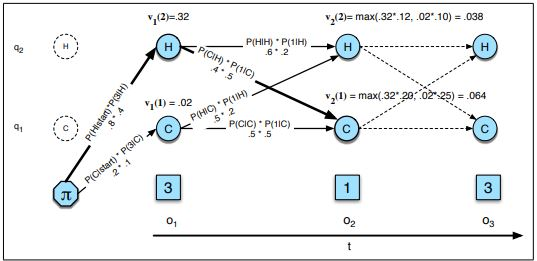
\includegraphics[width=18cm,height=8cm]{viterbi.JPG}
 \end{figure}
 \vspace{-1cm}
 \textit {Ví dụ thuật toán Viterbi}

Có T biến quan sát được, với mỗi biến quan sát tương ứng sẽ có K States cần duyệt, trong mỗi State cần liên hệ lại với K States của biến quan sát trước đó (Để thực hiện công thức quy hoạch động). Do đó độ phức tạp thuật toán là O(T.$K^2$)

\textbf{Câu 1: Cài đặt thuật toán Viterbi}

Tạo ra hai bảng hai chiếu có kích thước KxT được tạo ra(K là kích thước của Hidden states, T là kích thước của Observations):
\begin{itemize}
    \item  Bảng T1: mỗi phần tử $T_1[i,j]$ lưu xác suất của con đường có khả năng đi tới nhất cho tới hiện tại:
    
    \item Bảng T2: mỗi phần tử $T_2[i,j]$ lưu $x_{j-1}$  trữ con đường có khả năng đi tới cao nhất.
    \item Các hạng tử trong bảng T1 và T2 được điền theo thứ tự tăng dần của K.j+i
    \item $T_1[i,j] = max(T_1[k,j-1].A[k,i].B[i,y_i])$
    \item $T_2[i,j] = argmax_k(T_1[k,j-1].A[k,i].B[i,y_i])$
\end{itemize}


%https://warwick.ac.uk/fac/sci/masdoc/current/msc-modules/ma916/mlia/hmm/
\end{document}
